\chapter{Results}

\section{Camera Calibration}

In figure \ref{fig:gui} the multisensor calibration \gls{gui} is shown with a test result. One of the SICK LMS151 \gls{lidar}s was used as point of reference for the purpose of demonstration and to have a comparator point to the camera.
\begin{figure}[htp]
	
	\centering
	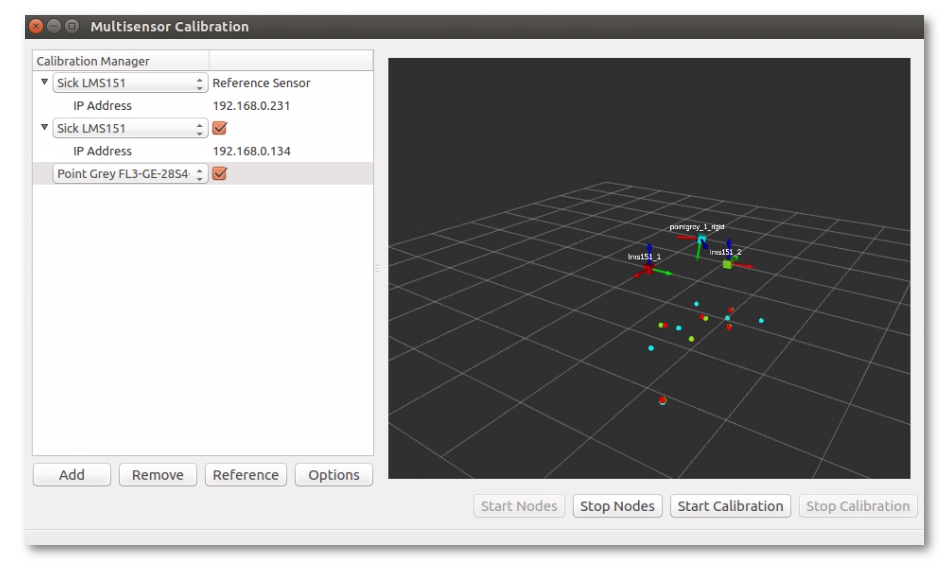
\includegraphics[width=0.9\textwidth]{capresults/imgs/gui.png}
	
	\caption{Calibration GUI with calibration result}
	\label{fig:gui}
	
\end{figure}

During the calibration procedure, the ball rolls in front of the camera and sensors. The range based sensors and the camera obtain a pointcloud of centroids of the ball during this activity. In the end, the transforms for each sensor are calculated, aligning the pointclouds of the several devices with each other. 

\begin{figure}
	\begin{center}
		\begin{lstlisting}[label={lst:calib_result}, caption={Calibration output file.},language=c++]
		-0.0563334  -0.998402 0.00440481   -1.07636
		0.997797 -0.0561436  0.0353294    1.08224
		-0.0350256 0.00638533   0.999366  0.0617893
		0          0          0          1	\end{lstlisting}
	\end{center}
\end{figure}

In listing \ref{lst:calib_result} an example output file of the calibration can be observed. The file contains a 4x4 matrix that indicates the transforms for the given sensor. Each sensor in the calibration will output its own file containing its transformation matrix relatively to the reference sensor. The reference sensor does not create a transform because it is assumed that this sensor is in the origin, unrotated. 

\section{Tracking}
\subsection{Dataset 1 - Highway / A25}
\subsection{Dataset 2 - Aveiro City Urban Area}